\documentclass[12pt]{article}

\usepackage{amsmath}
\usepackage{amssymb}
\usepackage[dvips]{graphicx}
\usepackage{eepic}
\usepackage{color}
\usepackage{wasysym} % \female \male
\usepackage[landscape,pdftex]{geometry}
\usepackage{fancyhdr}
\usepackage{wasysym} % for check symbol
\usepackage{hyperref}

\DeclareOption{bigsym}{\DeclareSymbolFont{largesymbols}{OMX}{psycm}{m}{n}}
\ProcessOptions

\hypersetup{pdfpagemode=UseNone} % don't show bookmarks on initial view
\hypersetup{colorlinks, urlcolor={white}}

\setlength{\oddsidemargin}{-0.75in}
\setlength{\evensidemargin}{-0.75in}
\setlength{\topmargin}{-1in}
\setlength{\textheight}{7.75in}
\setlength{\textwidth}{10.5in}
\setlength{\footskip}{0in}
\setlength{\parindent}{0pt}
\setlength{\rightskip}{0pt plus 1fil} % makes ragged right

\renewcommand{\familydefault}{phv} % helvetica

% following: color
\definecolor{mybgcolor}{rgb}{0,0,0.3125}
\definecolor{myyellow}{rgb}{1,1,0.4}
\definecolor{myblue}{rgb}{0.4,0.8,1}
\definecolor{mypink}{rgb}{1,0.4,1}
\definecolor{myhotpink}{rgb}{1,0,0.5}
\definecolor{mywhite}{rgb}{1,1,1}

% following: B/W
%\definecolor{mybgcolor}{rgb}{1,1,1}
%\definecolor{myyellow}{rgb}{0,0,0}
%\definecolor{myblue}{rgb}{0,0,0}
%\definecolor{mypink}{rgb}{0,0,0}
%\definecolor{myhotpink}{rgb}{0,0,0}
%\definecolor{mywhite}{rgb}{0,0,0}

% header/footer layout
\pagestyle{fancy}
\lhead{} \chead{} \rhead{}
\lfoot{} \cfoot{} \rfoot{\color{myyellow} \thepage}
\renewcommand{\headrulewidth}{0pt}
\renewcommand{\footrulewidth}{0pt}

% font sizes
\newcommand{\superlarge}{\fontsize{60}{60} \selectfont}
\newcommand{\titlesize}{\fontsize{40}{50} \selectfont}
\newcommand{\headsize}{\fontsize{35}{35} \selectfont}
\newcommand{\textsize}{\fontsize{30}{35} \selectfont}
\newcommand{\smallsize}{\fontsize{25}{30} \selectfont}
\newcommand{\smallersize}{\fontsize{20}{25} \selectfont}
\newcommand{\smallestsize}{\fontsize{18}{22} \selectfont}
\newcommand{\evensmaller}{\fontsize{14}{18} \selectfont}
\newcommand{\lod}{\text{LOD}}
\newcommand{\bic}{\text{BIC}}
\newcommand{\rss}{\text{RSS}}
\newcommand{\var}{\text{var}}
\newcommand{\M}{\text{M}}
%\renewcommand{\log}{\text{log}}
%\renewcommand{\max}{\text{max}}



\pagecolor{mybgcolor}
\color{mywhite}

\begin{document}

\thispagestyle{empty}

\begin{center}
\titlesize \color{myyellow}

\vspace*{19.5mm}

{\headsize How to display data badly}

\vspace*{19.5mm}

\color{mypink}
\rule{10in}{1mm}
%\vspace{-10mm}

\vspace{10mm}

\textsize \color{myblue}
Karl W Broman
\vspace{5mm}

{\smallersize Biostatistics \& Medical Informatics

University of Wisconsin -- Madison
\vspace{20mm}


\href{http://kbroman.org}{\tt kbroman.org} \\[5pt]
\href{https://github.com/kbroman}{\tt github.com/kbroman} \\[-5pt]
\href{https://twitter.com/kwbroman}{\tt @kwbroman}
}

\end{center}

\vfill \hfill
\href{http://creativecommons.org/publicdomain/zero/1.0/}{
\includegraphics[height=14mm]{Figs/cc-zero.png}}

\newpage

\thispagestyle{empty}

\begin{center}
\titlesize \color{myyellow}

\vspace*{10mm}

{\headsize Using Microsoft Excel to \\[12pt]
obscure your data and \\[2pt]
annoy your readers}


\color{mypink}
\rule{10in}{1mm}
%\vspace{-10mm}

\vspace{10mm}

\textsize \color{myblue}
Karl W Broman
\vspace{5mm}

{\smallersize Biostatistics \& Medical Informatics

University of Wisconsin -- Madison
\vspace{20mm}


\href{http://kbroman.org}{\tt kbroman.org} \\[5pt]
\href{https://github.com/kbroman}{\tt github.com/kbroman} \\[-5pt]
\href{https://twitter.com/kwbroman}{\tt @kwbroman}
}

\end{center}

\vfill \hfill
\href{http://creativecommons.org/publicdomain/zero/1.0/}{
\includegraphics[height=14mm]{Figs/cc-zero.png}}

\newpage

\headsize \color{myyellow}
\hfill 
\begin{minipage}{5.75in}
\centering
Inspiration
\end{minipage}

\vspace{30mm}

\color{mywhite}
\smallsize

\hspace{0.5in} \begin{minipage}{9in}
This lecture was inspired by

\vspace{10mm}

\hfill \begin{minipage}{8.5in}
{\smallersize \color{myblue}
H Wainer (1984) How to display data badly. American Statistician
38(2): 137--147}
\end{minipage}

\vspace{20mm}

Dr. Wainer was the first to elucidate the principles of the bad
display of data.

\vspace{20mm}

The now widespread use of {\color{mypink} Microsoft Excel} has
resulted in remarkable advances in the field.
\end{minipage}

\newpage

\headsize \color{myyellow}
\hfill \begin{minipage}{5.75in}
\centering
General principles
\end{minipage}

\vspace{10mm}
\smallsize \color{mywhite}

\hfill \begin{minipage}[t]{10in}
The aim of good data graphics:

\vspace{10mm}

\hfill \begin{minipage}{9.5in}
\smallersize
\color{myblue} Display data accurately and clearly.
\end{minipage}

\vspace{30mm}

Some rules for displaying data badly:

\vspace{8mm}

\hfill \begin{minipage}{9.6in}
\color{myblue} \smallersize
\begin{itemize}
\item Display as little information as possible.
\item Obscure what you do show (with chart junk).
\item Use pseudo-3d and color gratuitously.
\item Make a pie chart (preferably in color and 3d).
\item Use a poorly chosen scale.
\item Ignore sig figs.
\end{itemize}
\end{minipage}
\end{minipage}

\newpage


\headsize \color{myyellow}
\hfill \begin{minipage}{5.75in}
\centering
Example 1
\end{minipage}

\vspace{30mm}

\centerline{\includegraphics[height=6in]{Figs/fig1a.png}}




\newpage


\headsize \color{myyellow}
\hfill \begin{minipage}{5.75in}
\centering
Example 1
\end{minipage}

\vspace{30mm}

\centerline{\includegraphics[height=6in]{Figs/fig1b.png}}



\newpage


\headsize \color{myyellow}
\hfill \begin{minipage}{5.75in}
\centering
Example 1
\end{minipage}

\vspace{30mm}

\centerline{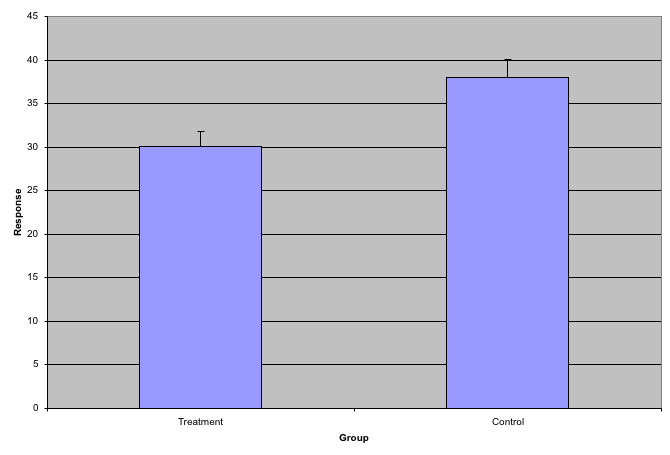
\includegraphics[height=6in]{Figs/fig1c.png}}


\newpage


\headsize \color{myyellow}
\hfill \begin{minipage}{5.75in}
\centering
Example 1
\end{minipage}

\vspace{30mm}

\centerline{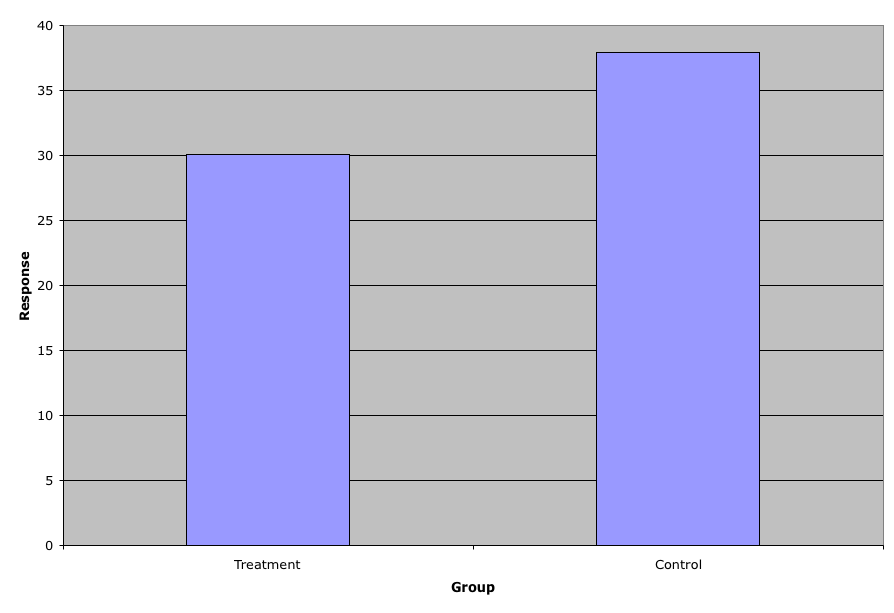
\includegraphics[height=6in]{Figs/fig1d.png}}


\newpage


\headsize \color{myyellow}
\hfill \begin{minipage}{5.75in}
\centering
Example 1
\end{minipage}

\vspace{30mm}

\centerline{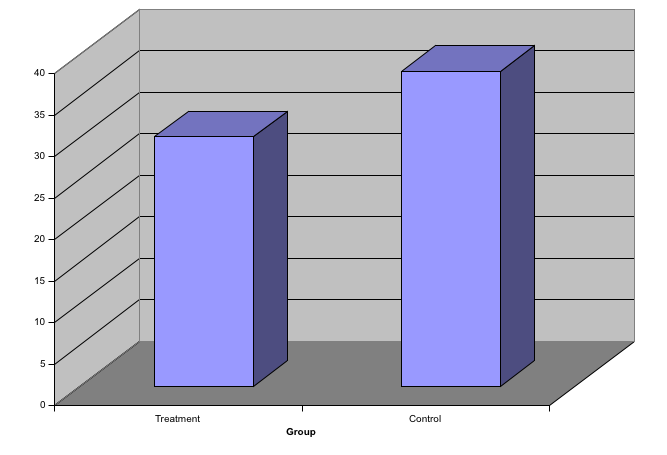
\includegraphics[height=6in]{Figs/fig1e.png}}


\newpage


\headsize \color{myyellow}
\hfill \begin{minipage}{5.75in}
\centering
Example 1
\end{minipage}

\vspace{30mm}

\centerline{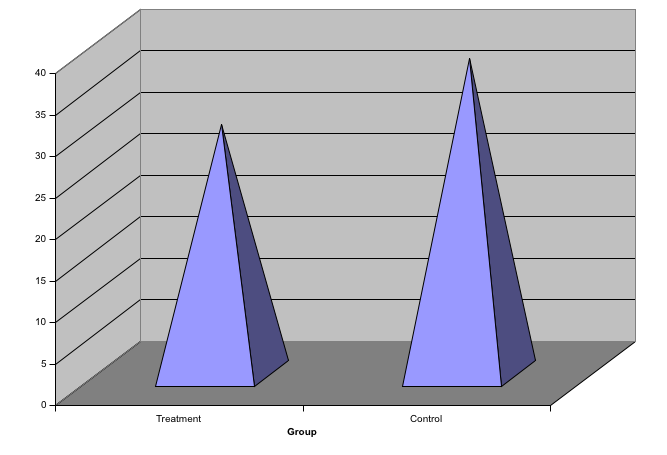
\includegraphics[height=6in]{Figs/fig1f.png}}


\newpage


\headsize \color{myyellow}
\hfill \begin{minipage}{5.75in}
\centering
Example 1
\end{minipage}

\vspace{30mm}

\centerline{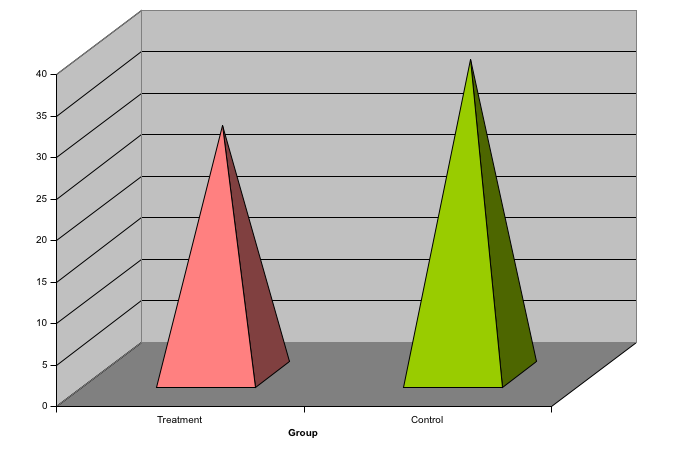
\includegraphics[height=6in]{Figs/fig1g.png}}


\newpage


\headsize \color{myyellow}
\hfill \begin{minipage}{5.75in}
\centering
Example 1
\end{minipage}

\vspace{30mm}

\centerline{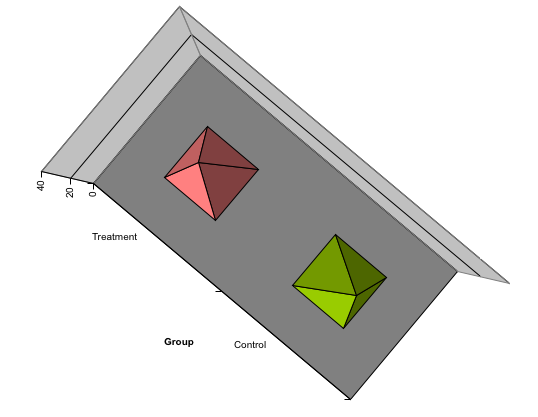
\includegraphics[height=6in]{Figs/fig1h.png}}



\newpage


\headsize \color{myyellow}
\hfill \begin{minipage}{5.75in}
\centering
Example 2
\end{minipage}

\vspace{30mm}

\centerline{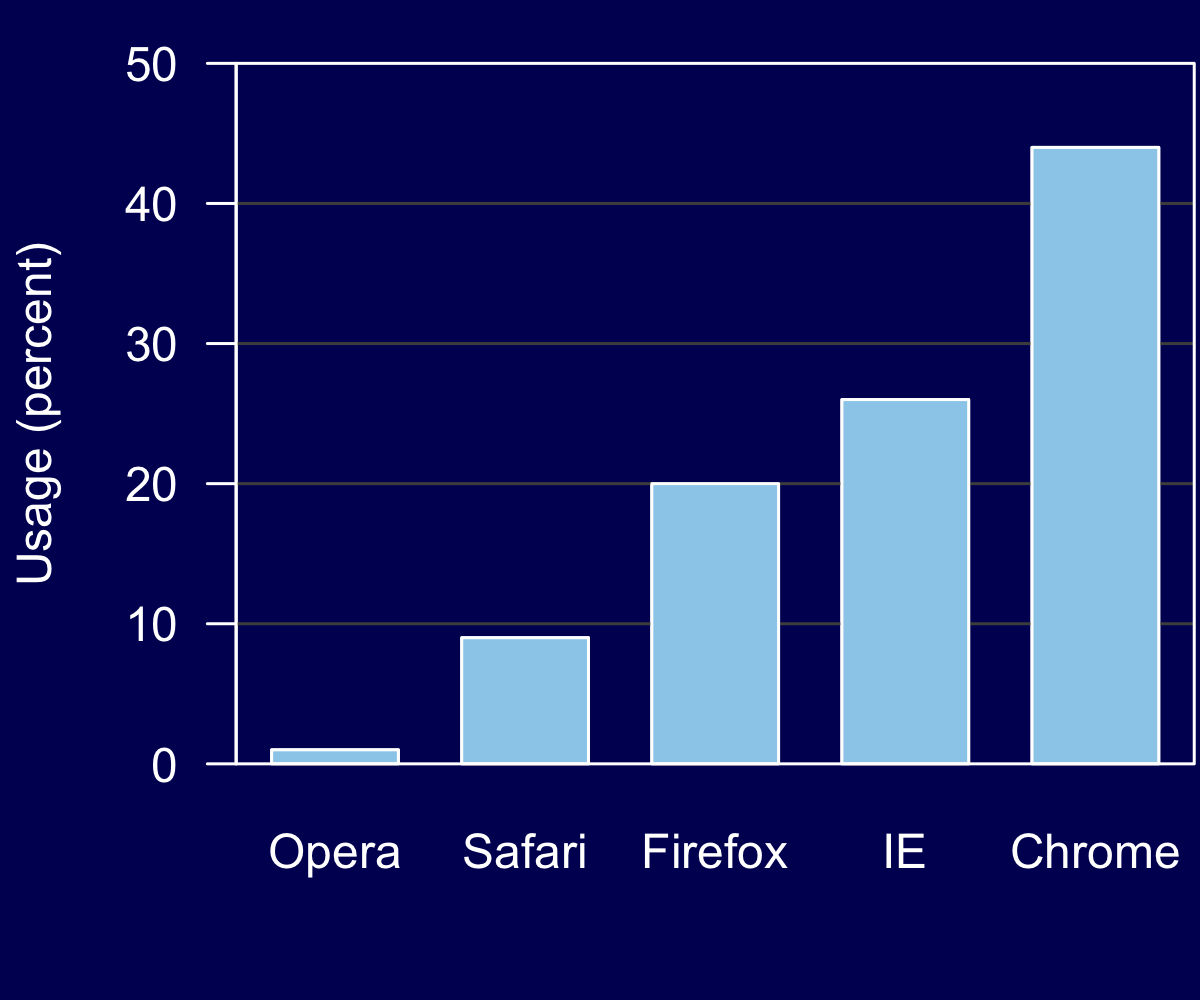
\includegraphics[height=6in]{Figs/fig2a_rev.png}}




\newpage


\headsize \color{myyellow}
\hfill \begin{minipage}{5.75in}
\centering
Example 2
\end{minipage}

\vspace{30mm}

\centerline{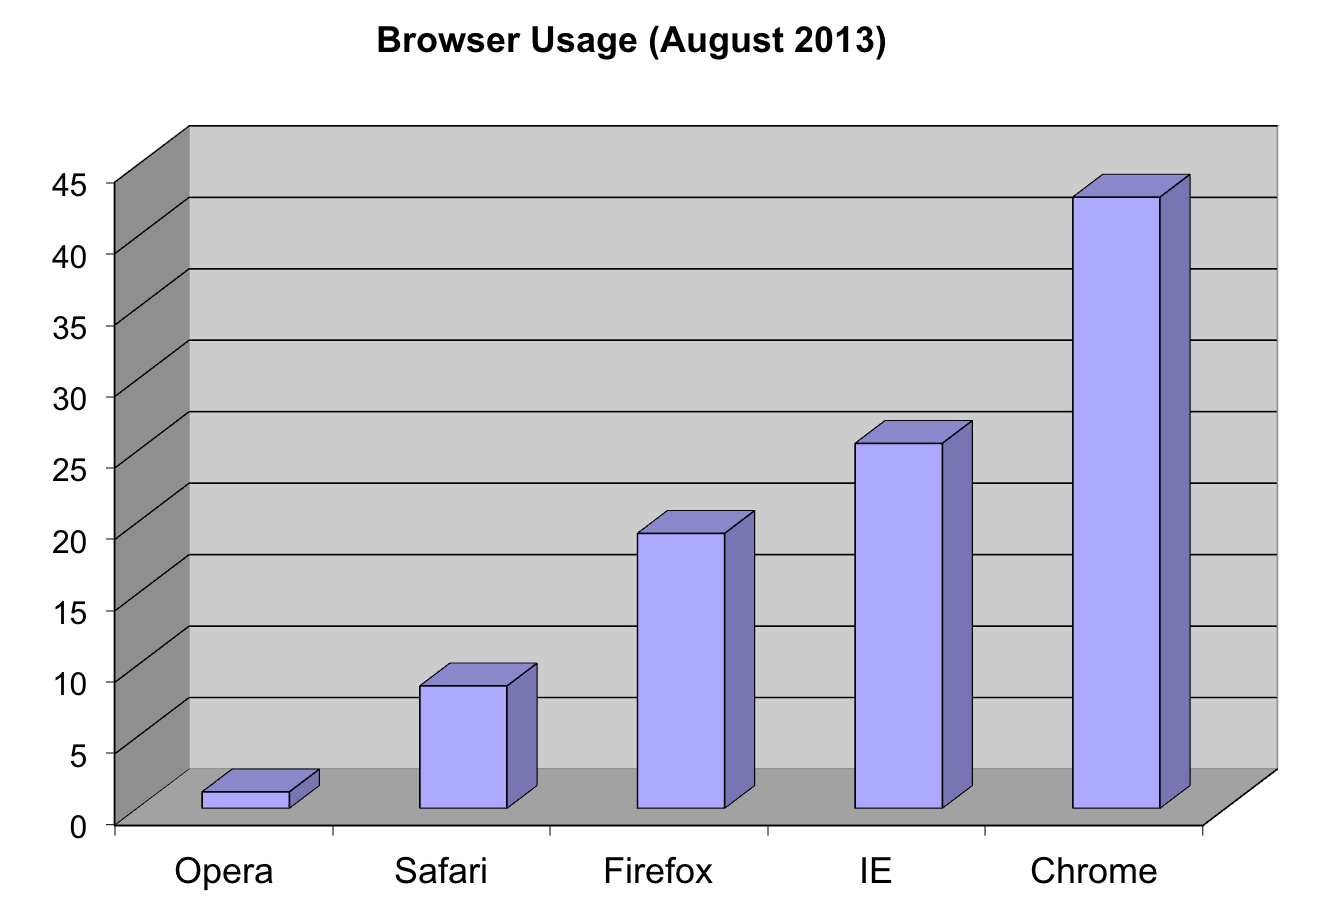
\includegraphics[height=6in]{Figs/fig2b.png}}



\newpage


\headsize \color{myyellow}
\hfill \begin{minipage}{5.75in}
\centering
Example 2
\end{minipage}

\vspace{30mm}

\centerline{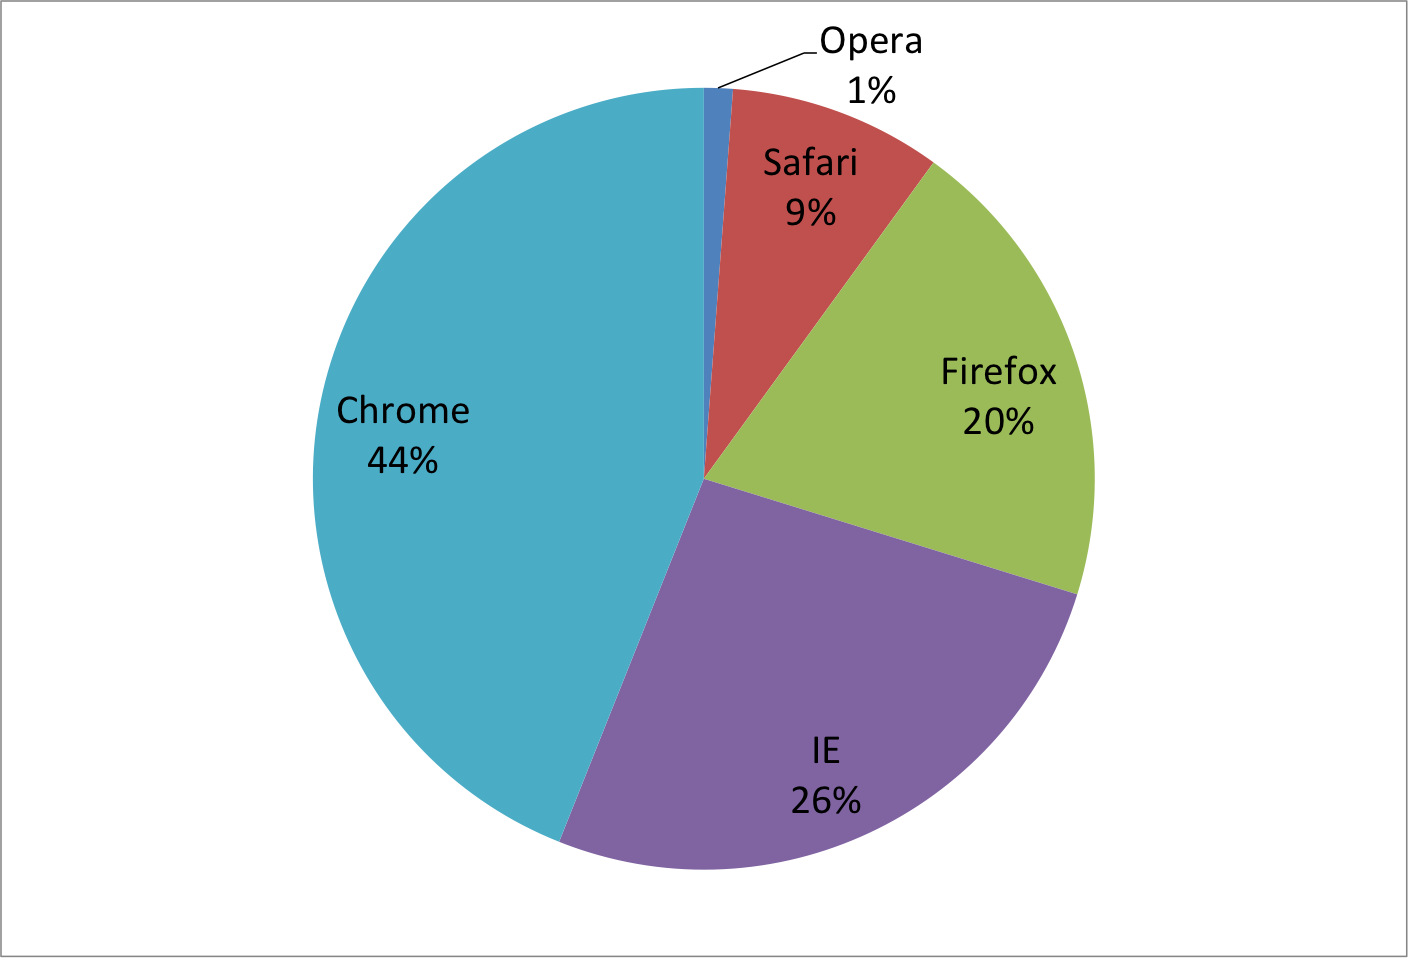
\includegraphics[height=6in]{Figs/fig2c.png}}


\newpage


\headsize \color{myyellow}
\hfill \begin{minipage}{5.75in}
\centering
Example 2
\end{minipage}

\vspace{30mm}

\centerline{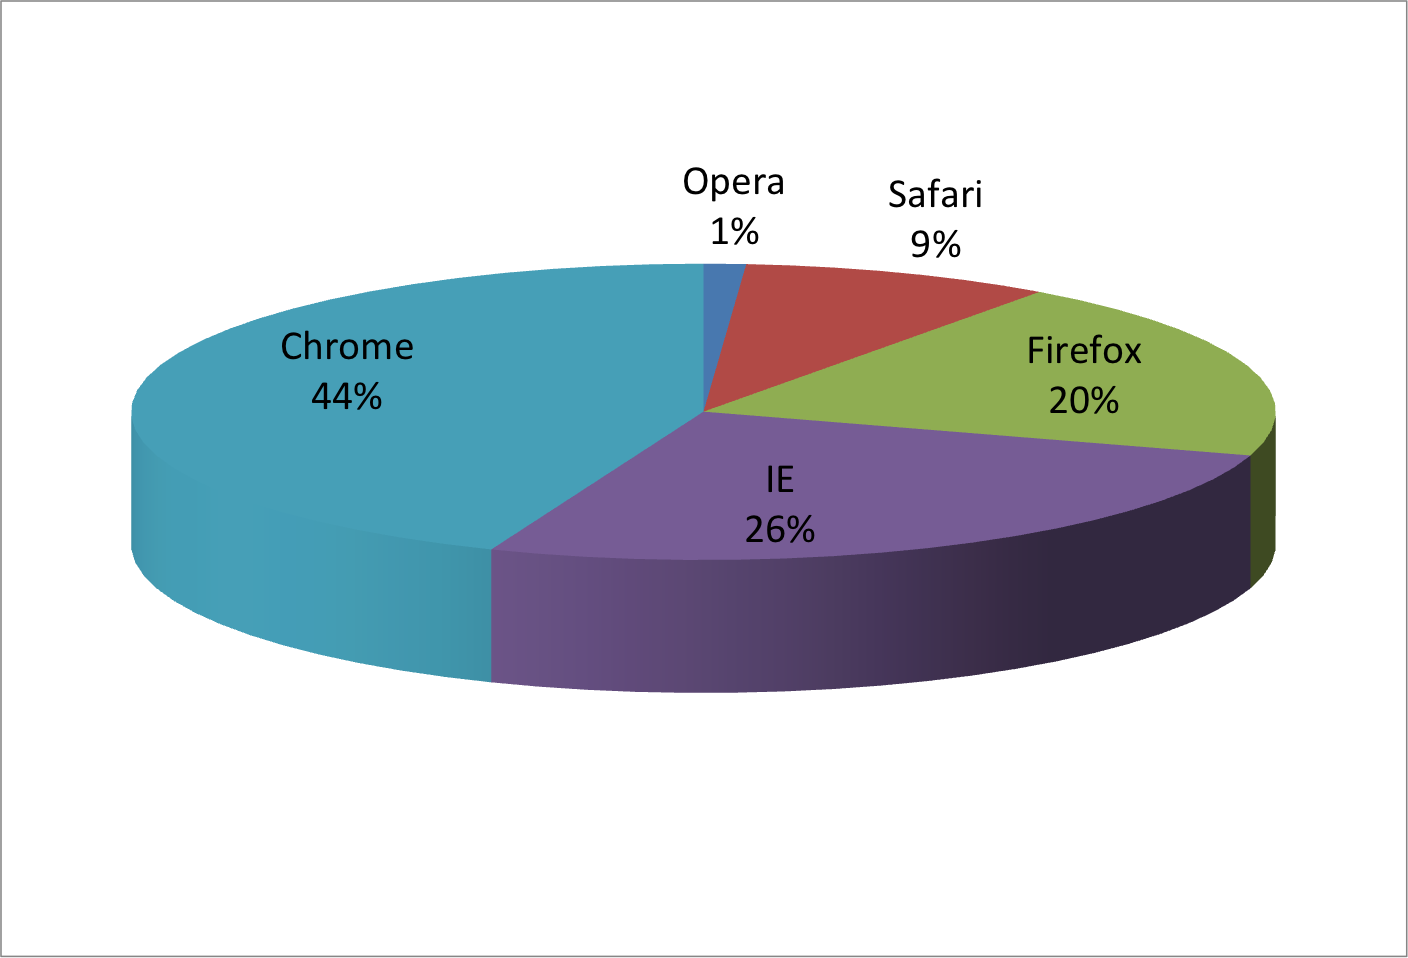
\includegraphics[height=6in]{Figs/fig2d.png}}


\newpage


\headsize \color{myyellow}
\hfill \begin{minipage}{5.75in}
\centering
Example 2
\end{minipage}

\vspace{30mm}

\centerline{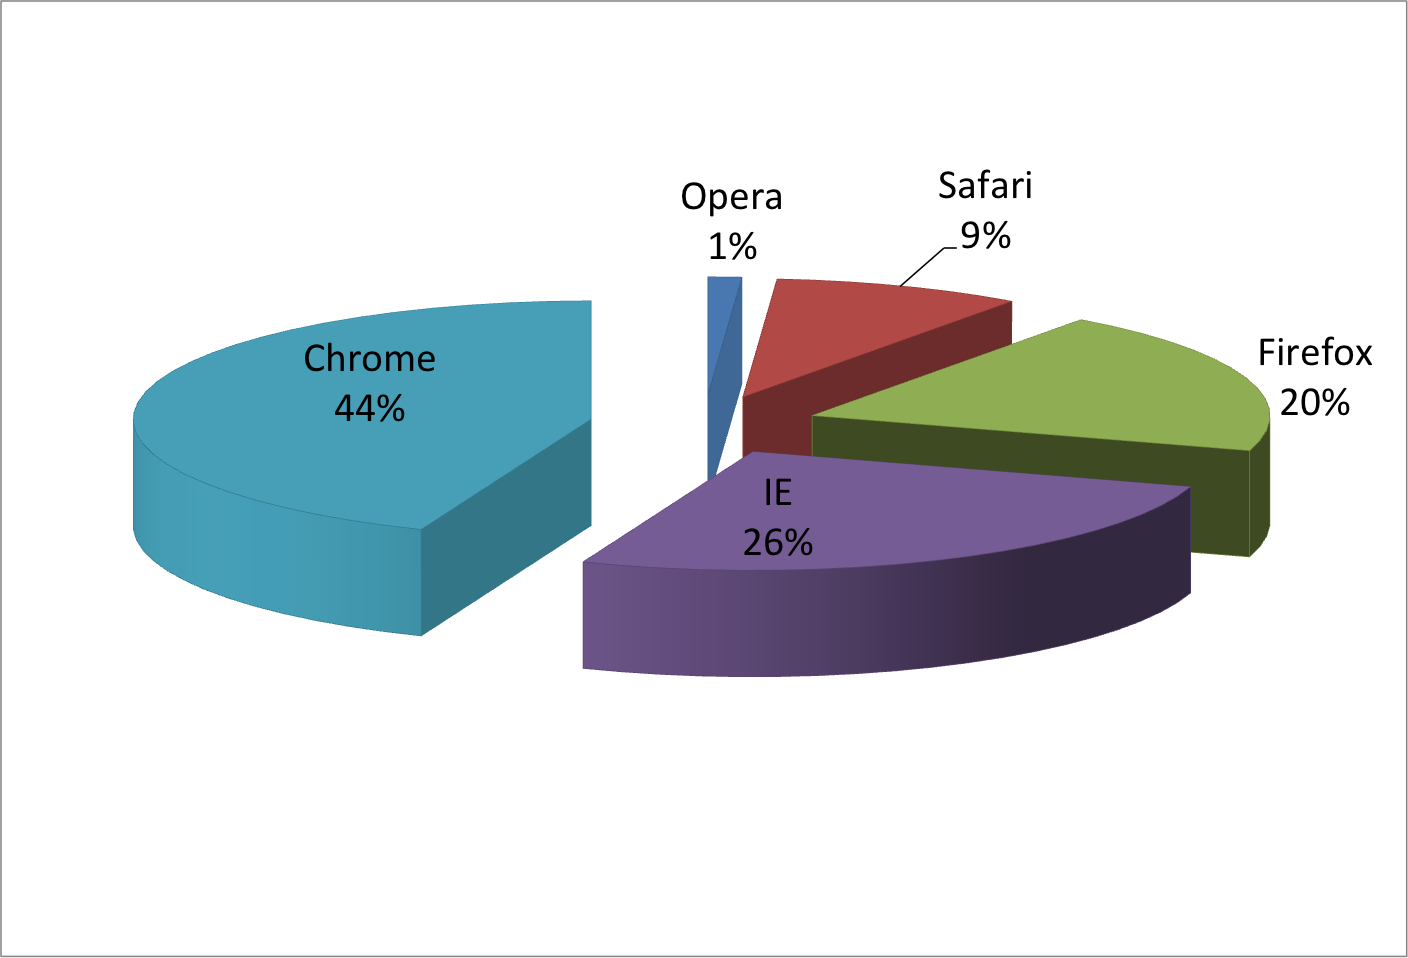
\includegraphics[height=6in]{Figs/fig2e.png}}



\newpage


\headsize \color{myyellow}
\hfill \begin{minipage}{5.75in}
\centering
Example 3
\end{minipage}

\vspace{30mm}

\centerline{\includegraphics[height=6in]{Figs/fig3a.png}}




\newpage


\headsize \color{myyellow}
\hfill \begin{minipage}{5.75in}
\centering
Example 3
\end{minipage}

\vspace{30mm}

\centerline{\includegraphics[height=6in]{Figs/fig3b.png}}



\newpage


\headsize \color{myyellow}
\hfill \begin{minipage}{5.75in}
\centering
Example 3
\end{minipage}

\vspace{30mm}

\centerline{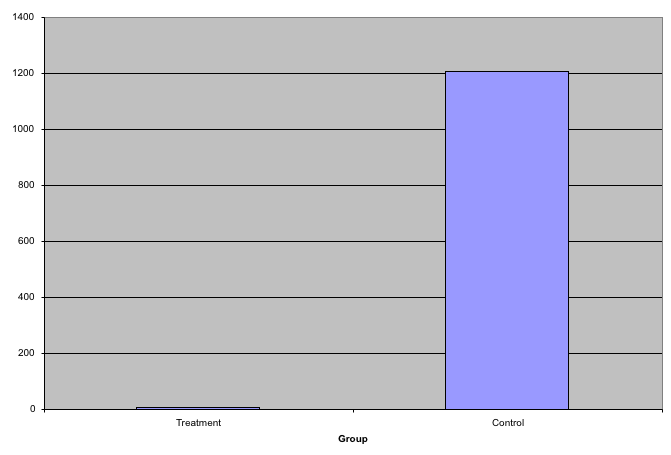
\includegraphics[height=6in]{Figs/fig3c.png}}


\newpage


\headsize \color{myyellow}
\hfill \begin{minipage}{5.75in}
\centering
Example 3
\end{minipage}

\vspace{30mm}

\centerline{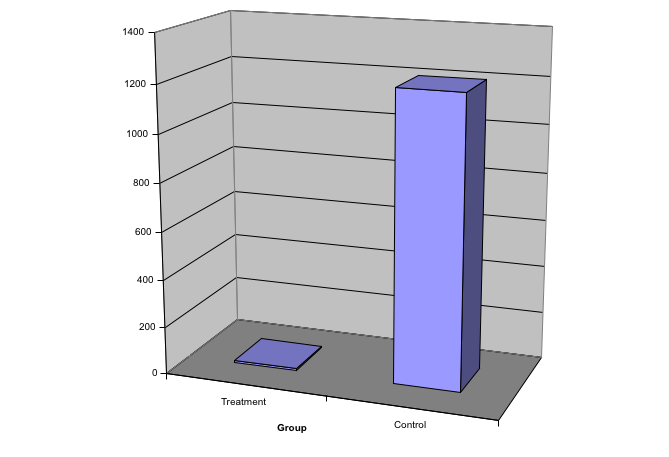
\includegraphics[height=6in]{Figs/fig3d.png}}

\newpage


\headsize \color{myyellow}
\hfill \begin{minipage}{5.75in}
\centering
Example 4
\end{minipage}

\vspace{30mm}

\centerline{\includegraphics[height=6in]{Figs/fig4a.png}}




\newpage


\headsize \color{myyellow}
\hfill \begin{minipage}{5.75in}
\centering
Example 4
\end{minipage}

\vspace{30mm}

\centerline{\includegraphics[height=6in]{Figs/fig4b.png}}



\newpage


\headsize \color{myyellow}
\hfill \begin{minipage}{5.75in}
\centering
Example 4
\end{minipage}

\vspace{30mm}

\centerline{\includegraphics[height=6in]{Figs/fig4c.png}}



\newpage


\headsize \color{myyellow}
\hfill \begin{minipage}{5.75in}
\centering
Example 5
\end{minipage}

\vspace{30mm}

\centerline{\includegraphics[height=6in]{Figs/fig5a.png}}




\newpage


\headsize \color{myyellow}
\hfill \begin{minipage}{5.75in}
\centering
Example 5
\end{minipage}

\vspace{30mm}

\centerline{\includegraphics[height=6in]{Figs/fig5b.png}}



\newpage


\headsize \color{myyellow}
\hfill \begin{minipage}{5.75in}
\centering
Example 5
\end{minipage}

\vspace{30mm}

\centerline{\includegraphics[height=6in]{Figs/fig5c.png}}


\newpage


\headsize \color{myyellow}
\hfill \begin{minipage}{5.75in}
\centering
Example 5
\end{minipage}

\vspace{30mm}

\centerline{\includegraphics[height=6in]{Figs/fig5d.png}}


\newpage


\headsize \color{myyellow}
\hfill \begin{minipage}{5.75in}
\centering
Example 5
\end{minipage}

\vspace{30mm}

\centerline{\includegraphics[height=6in]{Figs/fig5e.png}}


\newpage


\headsize \color{myyellow}
\hfill \begin{minipage}{5.75in}
\centering
Example 5
\end{minipage}

\vspace{30mm}

\centerline{\includegraphics[height=6in]{Figs/fig5f.png}}


\newpage


\headsize \color{myyellow}
\hfill \begin{minipage}{5.75in}
\centering
Example 6
\end{minipage}

\vspace{30mm}

\centerline{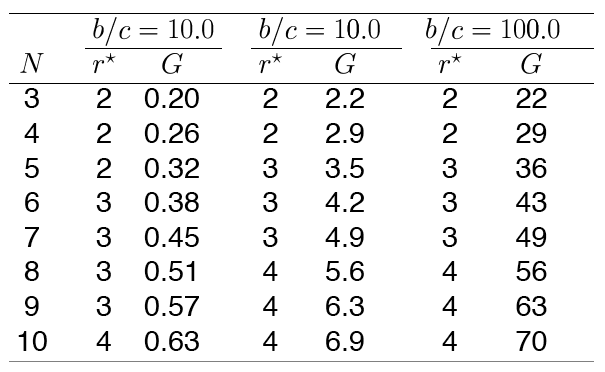
\includegraphics[height=5.5in]{Figs/tableA.png}}


\newpage


\headsize \color{myyellow}
\hfill \begin{minipage}{5.75in}
\centering
Example 6
\end{minipage}

\vspace{30mm}

\centerline{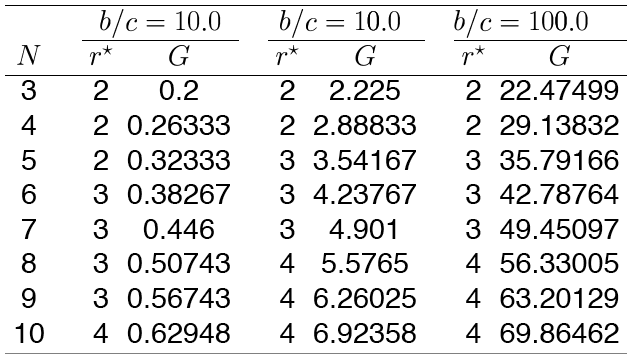
\includegraphics[height=5.5in]{Figs/tableB.png}}


\newpage


\headsize \color{myyellow}
\hfill \begin{minipage}{5.75in}
\centering
Example 7
\end{minipage}

\vspace{30mm}

\centerline{\includegraphics[height=5.5in]{Figs/fig8a.png}}


\newpage


\headsize \color{myyellow}
\hfill \begin{minipage}{5.75in}
\centering
Example 7
\end{minipage}

\vspace{30mm}

\centerline{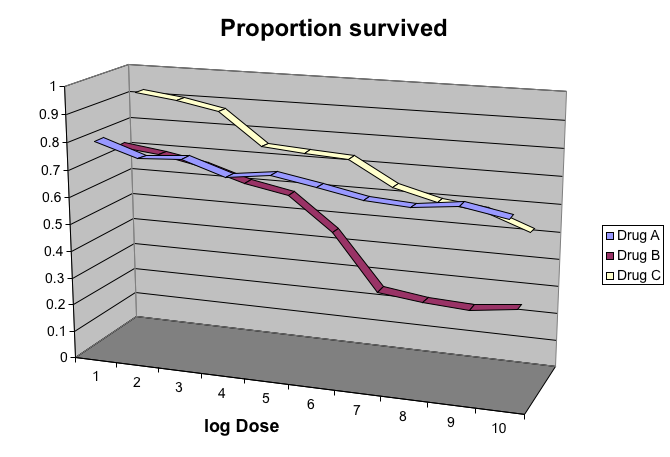
\includegraphics[height=5.5in]{Figs/fig8b.png}}




\newpage

\headsize \color{myyellow}
\hfill \begin{minipage}{5.75in}
\centering
Displaying data well
\end{minipage}

\vspace{30mm}
\smallsize \color{mywhite}

\hspace{0.5in} \begin{minipage}[t]{9in}
\begin{itemize}

\itemsep24pt

\item Be accurate and clear.

\item Let the data speak.

{\color{myblue} \smallersize
\begin{itemize}
\item Show as much information as possible, taking care not to
  obscure the message.
\end{itemize} }

\item Science not sales.

{\color{myblue} \smallersize
\begin{itemize}
\item Avoid unnecessary frills (esp. gratuitous 3d).
\end{itemize} }

\item In tables, every digit should be meaningful. Don't drop ending 0's.

\end{itemize}
\end{minipage}


\end{document}
